Далее для простоты и определённости рассматривается двумерный случай.
На случай больших размерностей все определения непосредственно переносятся.

Адаптивная сетка состоит из последовательности \emph{уровней} $l = 1, 2, \ldots, l_{\text{max}}$.
Каждый уровень представляет из себя набор прямоугольных областей $G_{l, m}$, где $l$ нумернует уровень, $m$~--- номер прямоугольной области (блока) на данном уровне.
Считаем, что на уровне $l$ находится $M_l$ блоков.
Общее множество, занимаемое уровнем $l$ есть
\begin{equation*}
    G_{l} = \bigcup_{m = 1}^{M_{l}} G_{l, m}
\end{equation*}
Уровень $l = 1$ будем называть основным, главным или корневым.
Этот уровень считаем состоящим из $M_{1} = 1$ прямоугольной области $[0, L_x] \times [0, L_y]$, которая дискретизуется равномерной сеткой:
\begin{equation*}
    \omega_{1, 1} = \left\{ (x_i, y_j) \mid x_i = (i - 1) * h_x, y_j = (j - 1) * h_y, i = 1, \ldots, N_x, j = 1, \ldots, N_y \right\}.
\end{equation*}
Каждый последующий уровень дискретизуется более мелкой сеткой, а именно шаг и по оси $x$ и по оси $y$ при переходе с уровня $l - 1$ на уровень $l$ уменьшается в $r_{l}$ раз.
Чаще всего рассматривают $r_{l} = 2, 4$.
В этой работе для определённости и простоты реализации расматривается фиксированный $r_l = 2 \quad \forall l > 1$.
Также на такую иерархию накладывается ограничение \emph{корректно-вложенных} уровней:
\begin{equation*}
    G_{l} \cap G_{l - 1} = G_{l}
\end{equation*}
то есть уровень $l + 1$ должен целиком лежать в уровне $l$.
(В ячеечном формализме это утверждение может быть сформулировано следующим образом: в окрестности каждой ячейки не должно быть ячеек, отличающихся от неё по размерам более чем в два раза).
Множество точек на каждом блоке нумеруется (локально) индексной системой координат $(i, j)$.
Таким образом, уровень $l$ должен хранить положения блоков $G_{l, 1}, \ldots, G_{l, M_{l}}$ в индексных координатах надблока уровня $l - 1$.
Пример корректной блочно-стурктурированной декартовой сетки приведён на \figref{fig:example_BSG}
\begin{figure}
    \centering
    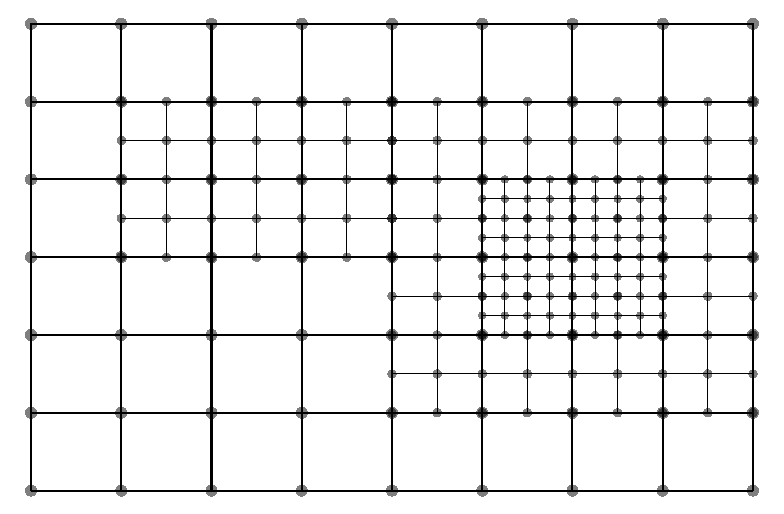
\includegraphics{Теория_блочных_локально_адаптивных_сеток/Топология_сетки/grid_topology.pdf}
    \caption{Пример корректной блочно-структурированной декартовой сетки}
    \label{fig:example_BSG}
\end{figure}
